\chapter*{Заключение}
\addcontentsline{toc}{chapter}{Заключение}
\label{ch:conclusion}

В результате выполнения практических работ была реализована полная модель системы цифровой связи, включающая:

\begin{itemize}
    \item Кодирование источника
    \item Помехоустойчивое кодирование
    \item Перемежение
    \item QPSK модуляцию
    \item OFDM модуляцию
    \item Модель канала с замираниями и шумом
    \item Демодуляцию и декодирование
\end{itemize}

Система демонстрирует устойчивую работу при наличии помех и многолучевого распространения. Реализованные алгоритмы обработки сигналов обеспечивают надёжную передачу данных в условиях реального канала связи.

\begin{figure}[ht]
    \centering
    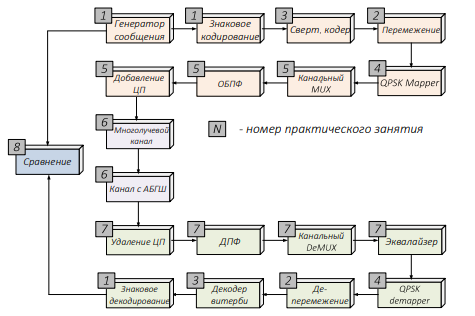
\includegraphics[width=0.8\textwidth]{system_overview.png}
    \caption{Обобщённая структура реализованной системы связи}
    \label{fig:system_overview}
\end{figure}
